\chapter{Azionamenti}
\paragraph{}
Il moto imposto al generico giunto del manipolatore è realizzato mediante un \emph{sistema di attuazione} che, in linea di principio, è costituito da:
\begin{itemize}
	\item una \emph{sorgente di alimentazione},
	\item un \emph{amplificatore di potenza},
	\item un \emph{servomotore},
	\item un \emph{organo di trasmissione}. 
\end{itemize}

Spieghiamo il funzionamento degli \emph{azionamenti elettrici} per l'attuazione dei giunti di un manipolatore. Partiamo dai \emph{modelli matematici} che descrivono il comportamento dinamico e successivamente ricaviamo gli \emph{schemi a blocchi} che consentono di evidenziare le caratteristiche di controllo.

Iniziamo col modello elettrico modellando il motore a corrente continua attraverso lo schema seguente,
\begin{center}
	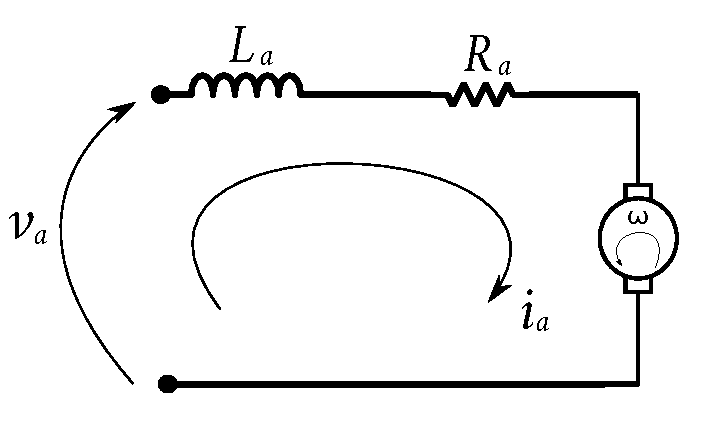
\includegraphics[scale=0.35]{circuitoMotore.pdf}
	\caption{Modello elettrico.}
\end{center}

scriviamo le equazioni che descrivono l'equilibrio elettrico del circuito nel dominio della variabile $s$,
\begin{equation}
	V_a = s L_a I_a + R_a I_a + k_v \Omega
\end{equation}
dove $V_a$ e $I_a$ rappresentano tensione e corrente applicate al circuito di armatura di resistenza $R_a$ e induttanza $L_a$, e $k_t \Omega$ rappresenta la forza controelettromotrice (FCEM) proporzionale alla velocità di rotazione $\Omega$ attraverso la costante di tensione $k_v$.

Proseguiamo col modello meccanico scrivendo le equazioni dell'equilibrio meccanico,
\begin{equation}
	\begin{cases}
		C_m = sI_m \Omega + F_m \Omega + D_l \\
		C_m = k_t I_a \\
	\end{cases}	
\end{equation}
dove $C_m$ rappresenta la coppia motrice elettromeccanica, $D_l$ il disturbo di coppia di carico, $I_m$ e $F_m$ sono il momento di inerzia e il coefficiente di attrito viscoso del motore e $k_t$ la costante di coppia, che in genere vale $k_t = k_v$.
\paragraph{}
Per quanto riguarda \emph{l'amplificatore di potenza}, ad esso viene associata la seguente relazione \emph{I/U}:
\begin{equation}
	\frac{V_a}{V_c} = \frac{G_v}{1 + sT_v}
\end{equation}
dove $G_v$ rappresenta il guadagno in tensione e $T_v$ una costante di tempo.
\paragraph{}
Lo schema a blocchi \emph{dell'amplificatore di potenza} e \emph{servomotore} è il seguente,
\begin{center}
	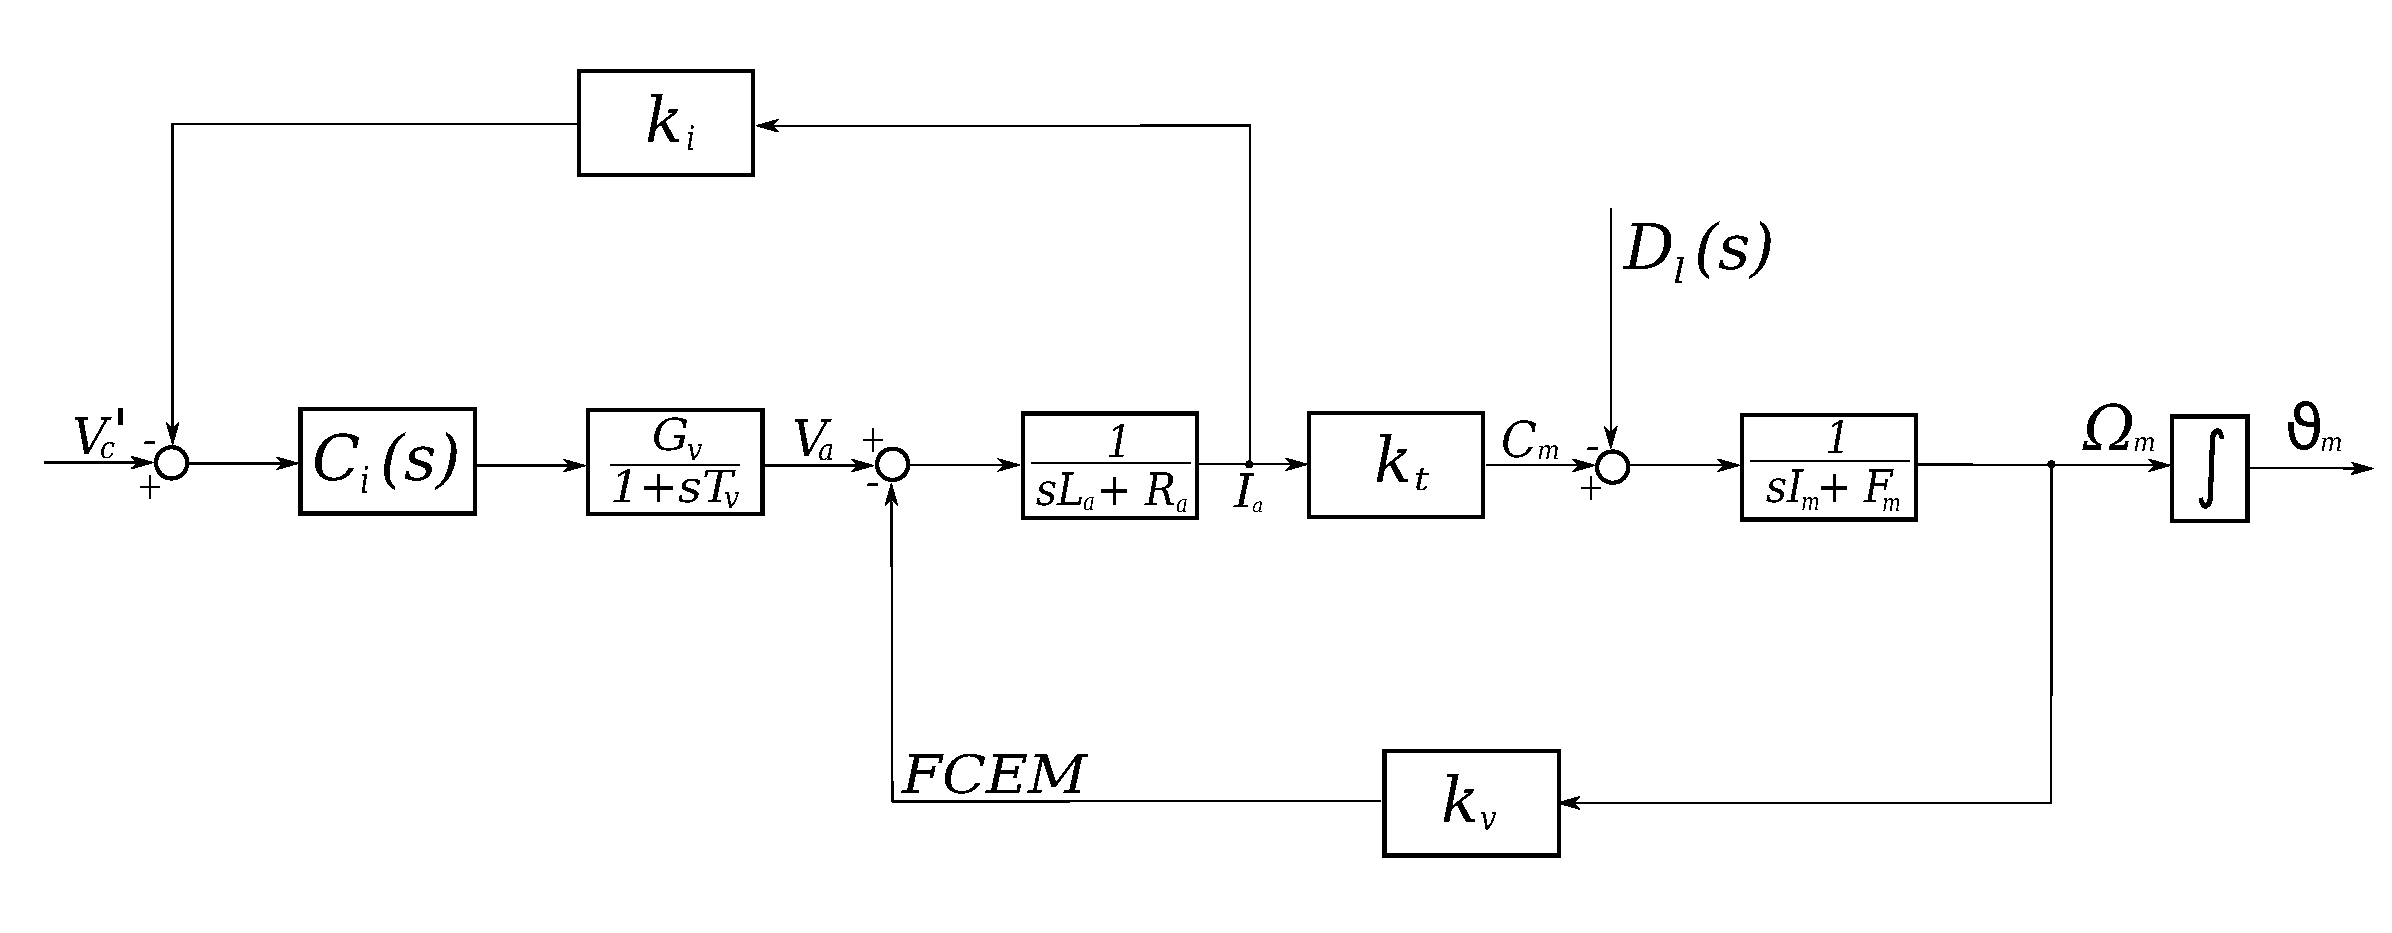
\includegraphics[scale=0.3]{schemaAzionamentoElettrico.pdf}
	\caption{Schema a blocchi di un azionamento elettrico.}
\end{center}
notiamo:
\begin{itemize}
	\item Vi è una \textbf{\emph{retroazione di corrente}} di armatura misurata tramite un trasduttore di costante $k_i$ inserito tra l'amplificatore di potenza e il circuito di armatura della macchina.
	\item Vi è un \textbf{\emph{regolatore di corrente}} $C_i(s)$ che consente di ottenere caratteristiche dell'azionamento particolari in base ai guadagni d'anello.
	\item $V'_c$ è un \textbf{\emph{riferimento di corrente}} e mediante un'opportuna scelta di $C_i(s)$ il ritardo tra corrente $I_a$ e tensione $V'_c$ risulta minore rispetto a quello tra $I_a$ e $V_c$.
\end{itemize}

\section{Pilotaggio}
Il pilotaggio di questo sistema può avvenire in due modi: \emph{pilotaggio in tensione} e \emph{pilotaggio in corrente}. 

\subsubsection{Pilotaggio in tensione}
Ricaviamo la \emph{funzione di trasferimento} considerando le seguenti equazioni e tralasciando il disturbo $D_l(s)$,
\begin{equation}
	\begin{cases}
		v_a(t) = L_a \frac{d i_a}{dt} + R_a i_a + k_v \omega \\
		c_m(t) = I_m \dot{\omega} + F_m \omega \\
		c_m(t) = k_t i_a \\
	\end{cases}
	\quad\longleftrightarrow\quad 
	\begin{cases}
		V_a(s) = (sL_a + R_a)I_a(s) + k_v \Omega(s) \\
		k_t I_a(s) = (sI_m + F_m) \Omega(s) \\
	\end{cases}
\end{equation}
ottenendo,
\begin{equation}
	\frac{\Omega(s)}{V_a(s)} = \frac{k_t}{(sL_a + R_a)(sI_m + F_m) + k_v k_t}
\end{equation}

Elaborando l'espressione della \emph{f.d.t} ottenuta eseguendo i prodotti e dividendo per $k_vk_t$ risulta
\begin{equation}
	\frac{\Omega(s)}{V_a(s)} = \frac{\frac{1}{k_v}}{\frac{L_a I_m s^2}{k_v k_t} + (\frac{R_a I_m}{k_v k_t} + \frac{L_a F_m}{k_v k_t})s + \frac{R_aF_m}{k_v k_t} + 1}
\end{equation}
e definiamo le seguenti costanti:
\begin{itemize}
	\item $\tau_m = \frac{R_a I_m}{k_v k_t}$ la \emph{costante di tempo meccanica}.
	\item $\tau_v = \frac{L_a}{R_a}$ la \emph{costante di tempo elettrica}.
	\item $\gamma = \frac{R_a F_m}{k_v k_t}$ parametro adimensionale con $\frac{k_vk_t}{R_a}$ \emph{attrito elettrico}.
\end{itemize}
ottenendo la riscrittura di ($7.6$)
\begin{equation}
	\frac{\Omega(s)}{V_a(s)} = \frac{\frac{1}{k_v}}{\tau_v \tau_m s^2 +  (\gamma \tau_v + \tau_m)s + \gamma +1}
\end{equation}
considerando $\gamma$ trascurabile (ad esempio nei motori commerciali $\gamma \ll 1$) otteniamo
\begin{equation}
	\frac{\Omega(s)}{V_a(s)} = \frac{\frac{1}{k_v}}{\tau_v \tau_m s^2 + \tau_m s + 1} = \frac{\frac{1}{k_v}}{(\tau_v s + 1)(\tau_m s + 1)}
\end{equation}
ottenendo due sistemi del primo ordine in serie.

Infine, quando la dinamica è molto veloce possiamo ottenere un'ulteriore approssimazione
\begin{equation}
	\frac{\Omega(s)}{V_a(s)} \approx \frac{\frac{1}{k_v}}{(\tau_m s + 1)}
\end{equation}

\subsubsection{Pilotaggio in corrente}
Ricaviamo la \emph{funzione di trasferimento} considerando le seguenti equazioni e tralasciando il disturbo $D_l(s)$,
\begin{equation}
	\begin{cases}
		c_m(t) = k_t i_a \\
		c_m(t) = I_m \dot{\omega} + F_m \omega \\
	\end{cases}
	\quad \longleftrightarrow \quad 
	\begin{cases}
		C_m(s) = k_t I_a(s) \\
		C_m(s) = (sI_m + F_m) \Omega(s) \\ 
	\end{cases}
\end{equation}
ottenendo
\begin{equation}
	\frac{\Omega(s)}{I_a(s)} = \frac{k_t}{sI_m + F_m}
\end{equation}

Elaborando l'espressione della \emph{f.d.t} ottenuta eseguendo la divisione dell'attrito $F_m$ risulta
\begin{equation}
	\frac{\Omega(s)}{I_a(s)} = \frac{\frac{k_t}{F_m}}{\frac{I_m}{F_m}s + 1}
\end{equation}
con $\frac{I_m}{F_m}$ costante di tempo meccanica.

\section{Azionamenti del sistema}
Esaminando lo schema in Figura $7.2$ notiamo che come già detto, la scelta del regolatore $C_i(s)$ dell'anello di corrente consente di ottenere, in base ai valori assunti dai guadagni d'anello, due tipi di azionamenti. 
\begin{itemize}
	\item \textbf{Azionamento in tensione} se $k_i = 0$.
	\item \textbf{Azionamento in corrente} se $k_i \neq 0$.
\end{itemize}

\subsubsection{\underline{Azionamento in tensione}}
In questo caso poniamo $k_i = 0$, supponiamo unitaria la costante di guadagno $C_i(s)$ e trascuriamo $D_l(s)$. 

Considerando che la frequenza di interesse è la \emph{bassa frequenza}, ciò implica le seguenti semplificazioni:
\begin{equation}
	\frac{1}{sL_a + R_a} \simeq \frac{1}{R_a}, \quad \frac{G_v}{sT_v + 1} \simeq G_v, \quad \frac{\frac{1}{k_v}}{s \tau_m + 1} \simeq \frac{1}{k_v}
\end{equation}

inoltre considerando che l'attrito meccanico viene trascurato rispetto l'attrito elettrico ($F_m \ll \frac{k_v k_t}{R_a}$)otteniamo,
\begin{equation}
	\begin{cases}
		V_a(s) = C_i(s) \frac{G_v}{sT_v + 1} V'_c \simeq G_v V'_c(s)\\
		C_m(s) = \frac{k_t}{R_a}\Bigl( G_v V'_c(s) - k_v \Omega(s) \Bigr) \\
		\Omega(s) = \frac{k_t}{R_a} \frac{1}{sI_m + F_m} \Bigl( G_v V'_c(s) - k_v \Omega(s) \\
	\end{cases}
\end{equation}
e scriviamo
\begin{equation}
	 \Omega(s) \Bigl( 1 + \frac{k_v k_t}{R_a} \frac{1}{sI_m + F_m} \Bigr) = \frac{k_t}{R_a} \frac{1}{sI_m + F_m} G_v V'_c(s)
\end{equation}
sviluppando il termine in parentesi ed eliminando i termini trascurabili (come $R_aF_m$), otteniamo la seguente espressione
\begin{equation}
	\Omega(s) \Bigl( R_a I_ms + k_v k_t \Bigr) = k_t G_v V'_c(s) \quad \Rightarrow \quad \Omega(s) = \frac{k_t}{R_a I_ms + k_v k_t} G_v V'_c(s)
\end{equation}
dividendo per $k_v k_t$ e considerando la \emph{bassa frequenza} otteniamo la seguente \emph{f.d.t.}
\begin{equation}
	\Omega(s) = \frac{\frac{1}{k_v}}{\frac{R_a I_m s}{k_v k_t} + 1} G_v V'_c(s) = \frac{\frac{1}{k_v}}{s\tau_m + 1} G_v V'_c(s) \simeq \frac{1}{k_v} G_v V'_c(s)
\end{equation}
e quindi l'azionamento assume caratteristiche di \emph{generatore controllato di velocità} espresso in figura,
\begin{center}
	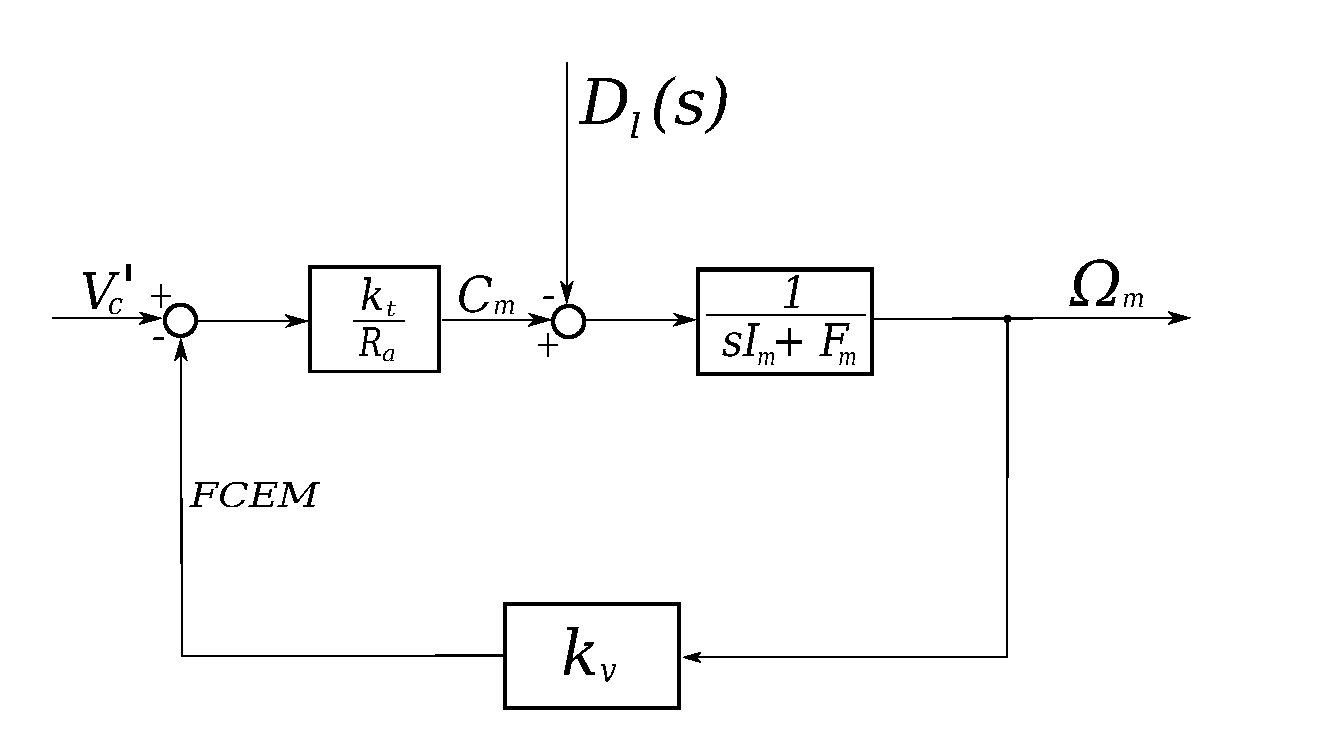
\includegraphics[scale=0.3]{schemaAzionamentoInTensione.pdf}
	\caption{Schema a blocchi dell'azionamento controllato in tensione.}
\end{center}

\subsubsection{\underline{Azionamento in corrente}}
In questo caso poniamo $k_i \neq 0$, supponiamo unitaria la costante di guadagno $C_i(s)$ così da avere \emph{un'azione integrale} e trascuriamo $D_l(s)$. La presenza di tale azione integrale ci da la possibilità di reiettare completamente a regime un disturbo di velocità costante. Infatti la FCEM $k_v \Omega(s)$ entra come un disturbo nell'anello di corrente.

Scriviamo la \emph{f.d.t.} di questo disturbo di velocità su $I_a(s)$
\begin{equation}
	\frac{I_a(s)}{k_v \Omega(s)} = \frac{-\frac{1}{R_a}}{1 + L(s)} = \frac{-\frac{1}{R_a}}{k_i C_i(s) \frac{G_v}{sT_v + 1} \frac{1}{R_a}}
\end{equation}
considerando le seguenti semplificazioni
\begin{itemize}
	\item $L(s)\vert_{s = 0} = \frac{G_v k_i}{R_a}$ dovuta alla \emph{bassa frequenza}.
	\item $G_v k_i \gg R_a$ a causa dell'elevato valore di $G_v$.
\end{itemize}
e otteniamo
\begin{equation}
	\frac{I_a(s)}{k_v \Omega(s)} \simeq \frac{\frac{1}{R_a}}{1 + G_v \frac{k_i}{R_a}} \simeq \frac{\frac{1}{R_a}}{G_v \frac{k_i}{R_a}} = \frac{1}{G_v k_i}
\end{equation}

Calcolando la \emph{f.d.t.} dell'anello di corrente con tutte le semplificazioni fatte sopra otteniamo
\begin{equation}
	\frac{I_a(s)}{V'_c(s)} = \frac{C_i(s) \frac{G_v}{sT_v + 1} \frac{1}{R_a}}{1 + k_i C_i(s) \frac{G_v}{s T_v + 1} \frac{1}{R_a}} \simeq \frac{1}{k_i}
\end{equation}
si ottiene un \emph{generatore controllato di coppia} espresso in figura,
\begin{center}
	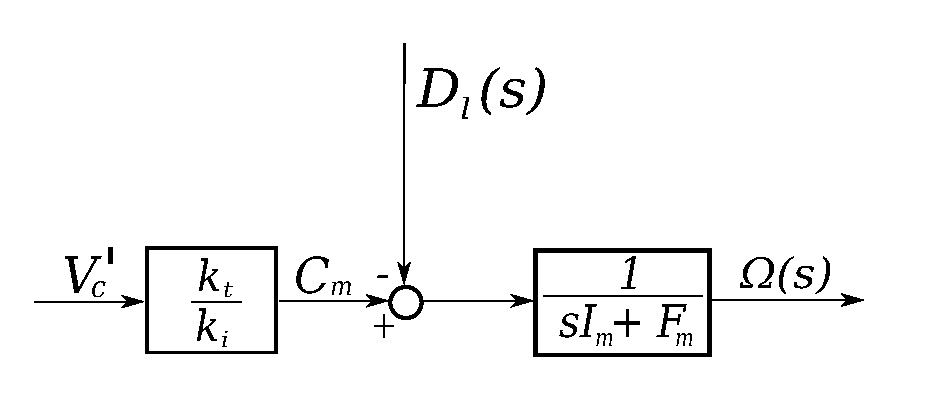
\includegraphics[scale=0.35]{schemaAzionamentoInCorrente.pdf}
	\caption{Schema a blocchi dell'azionamento controllato in corrente}
\end{center}

\section{Effetti del disturbo $D_l(s)$}
Fino adesso abbiamo trascurato il disturbo $D_l(s)$, andiamo a calcolarci l'effetto del disturbo di coppia $D_l(s)$ su $\Omega(s)$ distinguendo opportunamente i due casi.

\subsubsection{Azionamento con $k_i = 0$:}
Calcoliamo l'effettiva $\Omega(s)$ così da vedere l'effetto di $D_l(s)$,
\begin{equation}
	\Omega(s) = G_v V'_c \frac{\frac{1}{k_v}}{s \tau_m + 1} - D_l(s) \frac{\frac{1}{sI_m + F_m}}{1 + \frac{k_v k_t}{R_a (s I_m) + F_m}} = G_v V'_c \frac{\frac{1}{k_v}}{s \tau_m + 1} - D_l(s) \frac{R_a}{s R_a I_m + R_a F_m + k_v k_t}
\end{equation}
considerando che $R_aF_m$ è trascurabile, otteniamo
\begin{equation}
	\Omega(s) = G_v V'_c \frac{\frac{1}{k_v}}{s \tau_m + 1} - D_l(s) \frac{\frac{R_a}{k_vk_t}}{\frac{R_aI_m}{k_vk_t}s + 1}
\end{equation}
con $\frac{R_a}{k_vk_t}$ una quantità piccola e $\frac{R_aI_m}{k_vk_t} = \tau_m$.

Otteniamo così la \emph{f.d.t.} tra il disturbo e l'uscita
\begin{equation}
	\frac{\Omega(s)}{D_l(s)} = - \frac{\frac{R_a}{k_v k_t}}{s\tau_m + 1}
\end{equation}

\subsubsection{Azionamento con $k_i \neq 0$:}
Calcoliamo l'effettiva $\Omega(s)$ così da vedere l'effetto di $D_l(s)$,
\begin{equation}
	\Omega(s) = \frac{\frac{k_v}{k_i}}{sI_m + F_m} V'_c(s) - \frac{1}{sI_m + F_m} D(s) = \frac{\frac{k_t}{k_v} \frac{1}{F_m}}{s \frac{I_m}{F_m}+1} V'_c(s) - \frac{\frac{1}{F_m}}{s\frac{I_m}{F_m} + 1}D_l(s)
\end{equation}
con $\frac{1}{F_m} \gg \frac{R_a}{k_v k_t}$ e $\frac{I_m}{F_m} \gg \frac{R_a I_m}{F_m}$.

Otteniamo così la \emph{f.d.t.} tra il disturbo e l'uscita
\begin{equation}
	\frac{\Omega(s)}{D_l(s)} = - \frac{\frac{1}{F_m}}{s\frac{I_m}{F_m} + 1}
\end{equation}